%\section{Introducción Teórica del tema a tratar y Marco Teórico}
\label{sec:2_marcoteorico}

\subsection{Historia del RFID}

\begin{itemize}
\item \textbf{1860:} James Clerk Maxwell, físico escocés, predijo la existencia de ondas radio y postuló su uso.

\item \textbf{1886:} Un científico alemán, Heinrich Rudolf Hertz probó que rápidas variaciones de corriente 	eléctrica podían ser proyectadas en el espacio en forma de ondas de radio, similar a las ondas de luz, y que ,éstas, eran medibles y repetibles.

\item \textbf{1902:} Guglielmo Marconi, físico italiano, demostró la primera comunicación de larga distancia usando ondas radio, atravesando el Atlántico. Consistió en transmitir SOS en código Morse, en particular la letra S.

\item \textbf{1942 (Durante la II Guerra Mundial):} Los británicos desarrollaron el primer sistema etiquetado de RFID, el objetivo era discriminar rápidamente entre su propia flota de aviones y los escuadrones alemanes. Los aviones británicos incorporaban tags que contestaban a un lector con un código \textit{“I am a friend”}. Basado en el sistema de identificación \textit{IFF (Identity Friend or Foe)}.

\item \textbf{1960:} La necesidad de seguridad en los materiales nucleares condujo al desarrollo de una etiqueta RFID como el EAS \textit{(Electronic Article Surveillance)}.

\item \textbf{1977:} La necesidad de seguridad en los materiales nucleares condujo al desarrollo de una etiqueta RFID como el EAS \textit{(Electronic Article Surveillance)}.

\item \textbf{A partir de 1980:} Se focaliza en la comercialización de la RFID, desde nuevas aplicaciones a mejoras en el comportamiento y el coste de lectores, etiquetas y antenas. El éxito es evidente viendo la situación actual de la RFID.

\item \textbf{2000:} \textit{Auto-ID Center} focaliza todos sus esfuerzos en el desarrollo tecnológico para la 	implantación masiva de la tecnología RFID en la cadena de suministro, proporcionando un sustituto al código de barras. Posteriormente se convierte en EPC global para gestionar y desarrollar estándares.

\end{itemize}


\subsection{Identificación por radiofrecuencia}
En los años recientes, los sistemas de identificación por radiofrecuencia (\textit{RFID} por sus siglas en inglés) se han vuelto muy populares en distintas áreas de la industria tales como logística, industria manufacturera, control de acceso, y transporte. Este tipo de sistemas forma parte de los que se conocen como \textit{sistemas de identificación automática (Auto-ID)} \cite{rfid_handbook}, donde el uso más extendido se encuentra en el código de barras. Los tipos de \textit{Auto-ID} se muestran en la figura \ref{fig:tipos_rfid}.

\begin{figure}[H]
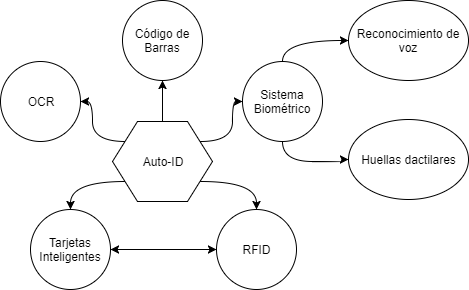
\includegraphics[scale=0.5]{tipos_rfid.png}
\centering
\caption{Tipos de Auto-ID}
\label{fig:tipos_rfid}
\end{figure}

La tecnología \textit{RFID} brinda información segura y permiten llevar un control eficiente del estado de los productos a muy bajo costo. El RFID nace como una evolución natural dedicada a identificar o realizar un seguimiento de personas, productos o animales. En comparación al código de barras, éste es capaz de almacenar más datos en memoria y permite la intercomunicación simultanea de varios \textit{tags}. Un sistema RFID está compuesto generalmente por un interrogador o lector (\textit{PCD - Proximity Coupling Device}) y uno o varios transponders, que generalmente toma la forma de tarjetas personales y/o tarjetas adhesivas (\textit{PICC - Proximity Integrated Circuit Card}). Cada transponder (\textit{tag}) cumple el rol de portador de información, tales como datos o identificación de un producto. Debido a su reducido tamaño y peso son dispositivos ideales para ser transportados por personas y animales, o para ser adheridos en algún producto.

Los transponders RFID se pueden clasificar en dos tipos debido a la de su alimentación: Activos o Pasivos. Los tags activos requieren energía adicional para alimentar el circuito, y los pasivos no requieren alimentación externa para su funcionamiento. 

Un ejemplo de los tags pasivos puede ser la tarjeta \textit{SUBE (Sistema Único de Boleto Electrónico)}. La SUBE es un sistema implementado en la República Argentina a partir del año 2011 que permite a cada usuario con su respectiva tarjeta inteligente, abonar los viajes en colectivos, subtes, trenes y los peajes adheridas a la Red SUBE. Éstas tarjetas cumplen con la norma ISO 14443-A que se describirán en la sección \ref{sec:iso}.



\subsection{Clasificación y estandarización de los sistemas RFID}

Existe una gran variedad de organizaciones que han determinado los estándares para la Identificación por Radio Frecuencia (RFID) según intereses, aplicaciones o simplemente por globalización. Entre las más destacadas encontramos la \textit{ISO (International Organization for Standardization)}, \textit{IEC (International Electrotechnical Commission)}, \textit{ASTM (American Society for Testing and Materials)} o \textit{EPCglobal (Asociación entre EAN International y GS1 Uniform Code Council)}.

También existen algunos sectores industriales que han establecido guías, ya sea para una mejor adaptación a sus realidades particulares, o bien porque no existían. Algunos ejemplos de estas industrias los encontramos en la \textit{FSTC (Financial Services Technology Consortium)}, el \textit{ICAR (International Committee for Animal Recording), CompTIA (Computer Technology Industry Association)}, la \textit{IATA (International Air Transport Association)}, \textit{EMV Contactless (Europay, Mastercard y Visa)}, organizaciones gubernamentales, etc.

\subsubsection{Regulación del espectro electromagnético}

Los distintos países han asignado diferentes zonas del espectro radioeléctrico para la RFID,  sin embargo, la mayoría de los países han acordado utilizar para los \textbf{sistemas de baja frecuencia (LF)} las zonas de 125 y 134,2 kHz del espectro, y la frecuencia de 13,56 MHz para los sistemas de \textbf{alta frecuencia (HF)}. Pero los \textbf{sistemas de ultra alta frecuencia (UHF)}, existen solo desde la segunda mitad de la década de los años 90 y los países no han acordado una sola zona del espectro para dicha banda, de manera que es mas complejo satisfacer óptimamente todos los requerimientos de los mercados existentes y/o potenciales.

En la Tabla \ref{table:rango_frec} se observa la diversidad de rangos del espectro UHF utilizados en diferentes países y regiones del mundo, mientras que en las bandas LF y HF se utilizan las mismas frecuencias.

\begin{table}[H]
\centering
\caption{Clasificación y rango de frecuencias}
\label{table:rango_frec}
\begin{tabular}{c|c|c|c}
\textbf{País o Región} & \textbf{LF}       & \textbf{HF} & \textbf{UHF}                                                                                \\ \hline
USA                    & 125 $-$ 134,2 kHz & 13,56 MHz   & 902 $-$ 928 MHz                                                                             \\
Europa                 & 125 $-$ 134,2 kHz & 13,56 MHz   & 865 $-$ 868 MHz                                                                             \\
Japón                  & 125 $-$ 134,2 kHz & 13,56 MHz   & 952 $-$ 954 MHz                                                                             \\
China                  & 125 $-$ 134,2 kHz & 13,56 MHz   & \begin{tabular}[c]{@{}c@{}}B1 = 840,5 $-$ 844,5 MHz\\ B2 = 920,5 $-$ 924,5 MHz\end{tabular} \\
Argentina              & 125 $-$ 134,2 kHz & 13,56 MHz   & 902 $-$ 928 MHz                                                                            
\end{tabular}
\end{table}

\subsubsection{Estándares establecidos}

Las familia de normas \textbf{ISO 18000} se han desarrollado para garantizar la interoperabilidad entre los sistemas RFID. Es el estándar que describe las diferentes tecnologías y/o frecuencias para la gestión a nivel de artículos. Las diferentes partes de este estándar describen la interface de comunicación vía aire de las distintas frecuencias para establecer los distintos comportamientos físicos.

Las distintas partes son:
\begin{itemize}
\item \textbf{Parte 1}: Arquitectura de referencia y definición de los parámetros estandarizados.
\item \textbf{Parte 2}: Parámetros establecidos para la interface de comunicación vía aire aplicados a los sistemas que funcionan a 135 KHz.
\item \textbf{Parte 3}: Parámetros establecidos para la interface de comunicación vía aire aplicados a los sistemas que funcionan a 13,56 MHz.
\item \textbf{Parte 4}: Parámetros establecidos para la interface de comunicación vía aire aplicados a los sistemas que funcionan a  2,45 GHz.
\item \textbf{Parte 5}: Parámetros establecidos para la interface de comunicación vía aire aplicados a los sistemas que funcionan a 5,8 GHz (fue retirada por falta de uso).
\item \textbf{Parte 6}: Parámetros establecidos para el interface de comunicación vía aire aplicados a los sistemas que funcionan entre 860 MHz y 960 MHz.
\item \textbf{Parte 7}: Parámetros establecidos para el interface de comunicación activo vía aire aplicados a los sistemas que funcionan a 433 MHz.
\end{itemize}

\subsubsection{Estándares LF}

\begin{itemize}
\item \textbf{ISO 14223} - Es el estándar que especifica la estructura del código de radiofrecuencia (RF) para transponders usados en animales. Esta norma es una extensión de los otros estándares \textbf{ISO 11784} e \textbf{ISO 11785}.
\item \textbf{ISO 11784} - Especifica la estructura del código de identificación
\item \textbf{ISO 11785} - Especifica la interface de comunicación vía aire aplicados a los sistemas que funcionan a 134,2 KHz, en la cual se definen y aprueban dos sistemas de intercambio de información: \textit{FDX-B (Full duplex)} y \textit{HDX (Half duplex)}.
\end{itemize}

\subsubsection{Estándares HF} 

\begin{itemize}
\item \textbf{ISO 14443} - Es el estándar basado en la frecuencia de 13,56 MHz \textit{(HF)} y es conocido como el estándar de tarjetas de proximidad o tarjetas con circuito integrado sin contacto.
\item \textbf{ISO 15692} - Protocolo de los datos usados en el intercambio de información en los sistemas RFID para la gestión de ítems, operando con el proceso de datos y la presentación en el tag RFID, así como el procesamiento inicial de los datos capturados desde transponder.
\item \textbf{ISO 15693} - Este estándar está basado también en la frecuencia de 13,56 MHz \textit{(HF)} y es conocido como el estándar para las tarjetas de vecindad \textit{(vicinity cards)}. La diferencia principal es la distancia de lectura/escritura que este estándar regula llegando a alcanzar 1,5 metros de distancia. Una de las claves de esta mayor distancia respecto a las tarjetas de proximidad (ISO 14443) es el campo magnético necesario para su activación, siendo de 0,15 a 5 A/m (1,5 a 7,5 A/m para la ISO 14443).
\item \textbf{ISO 18092} - Estándar que describe el intercambio de información sin contacto entre sistemas, conocido también como \textit{NFC (Near Field Communication – interface y protocolo NFCIP-1)}.
\item \textbf{ISO 21481} - Sistemas de intercambio de información y telecomunicaciones entre sistemas, \textit{Near Field Communications interface y protocolo – 2 (NFCIP-2)}.
\item \textbf{EMV Contactless} - Especificaciones para los sistemas de pago que define la arquitectura y requisitos generales, puntos de partida, especificaciones del kernel y el protocolo de comunicaciones contactless. Se basa en la \textbf{ISO 7816} y la \textbf{ISO 14443}.
\end{itemize}

\subsubsection{Estándares UHF}

\begin{itemize}
\item \textbf{ISO 18000-6} - Especifica los requisitos físicos y lógicos para un sistema de retrodispersión pasiva (passive-backscatter). El Lector recibe información de una etiqueta transmitiendo una señal de RF de onda continua (CW) a la etiqueta; la etiqueta responde modulando el coeficiente de reflexión de su antena, con lo cual retrodispersa una señal de información al Lector. 
\item \textbf{ISO 18000-61 – Type A} - El sistema es \textit{ITF (Interrogator-Talks-First)}, lo que significa que una etiqueta modula su coeficiente de reflexión de la antena con una señal de información solo después de ser dirigido por un Lector. Las etiquetas del tipo A utilizan la codificación \textit{PIE (Pulse-Interval Encoding)} en el enlace directo, y el algoritmo anti-colisión llamado \textit{ALOHA}.
\item \textbf{ISO 18000-62 – Type B} - El sistema es \textit{ITF} como las del tipo A, pero utiliza Codificación Manchester en el enlace directo, y como algoritmo anti-colisión \textit{binary-tree}.
\item \textbf{ISO 18000-63 – Type C} - El sistema es \textit{ITF} y utiliza Codificación \textit{PIE} como las de tipo A, pero como algoritmo anti-colisión utiliza \textit{random slotted}.
\item \textbf{ISO 18000-64 – Type D} - El sistema es \textit{TOTAL (Tag Only Talks After Listening)}, lo que significa que una etiqueta modula su coeficiente de reflexión de antena con una señal de información al ingresar al campo de un Lector, después de escuchar por primera vez la modulación del Lector para determinar si el sistema es o no ITF. La codificación de las etiquetas del tipo D es por posición de pulso \textit{(Pulse Position Encoding)} o \textit{Miller M = 2}.
\item \textbf{EPC UHF Class1 Gen2} – Las etiquetas \textit{RFID EPC} Clase 1 Gen-2 se utilizan para identificar un artículo en la cadena de suministro a nivel mundial. "Clase 1" se refiere a la funcionalidad de la etiqueta, mientras que "Gen-2" se refiere a los estándares físicos y lógicos de la etiqueta y el sistema abarcador. Estos estándares son mantenidos por \textit{EPCglobal}. 
\end{itemize}

\subsection{Norma ISO/IEC 14443} \label{sec:iso}

ISO/IEC 14443 es un estándar internacional relacionado con las tarjetas de identificación por radiofrecuencia (RFID), en especial para las tarjetas de proximidad, gestionado conjuntamente por la Organización Internacional de Normalización (ISO) y Comisión Electrónica Internacional (IEC).

Ésta norma consiste en 4 partes:
\begin{itemize}
	\item \textbf{Parte 1:} Especifica las características físicas.
	\item \textbf{Parte 2:} Especifica la potencia RF, los distintos tipos de modulación y la interfaz con el \textit{core} digital.
	\item \textbf{Parte 3:} Especifica la inicialización y anticolisión entre los chips.
	\item \textbf{Parte 4:} Especifica el protocolo de transmisión de datos. 
\end{itemize}

\subsection{Norma ISO/IEC 14443 Parte 1: Características físicas}

Ésta primera parte, al comienzo define los símbolos y abreviaciones que se utilizará a lo largo de la norma. Entre ellas, las más relevantes son:

\begin{itemize}
	\item \textbf{Proximity Integrated Circuit Card (PICC)}: Es el dispositivo portador de la información, generalmente tiene forma de tarjeta \textit{(tag)}.
	\item \textbf{Proximity Coupling Device (PCD)}: Es el dispositivo que produce el campo magnético y comunica con el PICC a través de acoplamiento inductivo.
\end{itemize}

En cuanto a características físicas, se define el tamaño y forma que tiene que tener la antena (86 x 54 x 3) mm, ya que la interfaz de radiofrecuencia y los bancos de prueba, que están definidos en la norma ISO/IEC 10373-6, son para una antena del tamaño de una tarjeta ID-1. El estándar ISO/IEC 7810 define el tamaño de éste tipo de tarjetas.

También se incluye información acerca de la radiación ultravioleta, rayos X, y temperaturas de operación para la PICC.

\subsection{Norma ISO/IEC 14443 Parte 2: Alimentación e interferencia de la señal de RF}
\label{sec:Norma14443-2}
En ésta segunda parte se especificará la naturaleza y las características de los campos que deben proveerse para alimentar y poder establecer una comunicación bidireccional entre el dispositivo de acoplamiento (\textit{PCD}) y las tarjetas de proximidad (\textit{PICC}). Como introducción sólo se presentará la interfaz de comunicación tipo A \cite{nfc_spec}.

\subsubsection{Términos y definiciones} 
\begin{itemize}
\item \textbf{Duración del bit:} Tiempo durante el cual un estado lógico es definido, al finalizar este un nuevo bit comienza.
\item \textbf{Modulación binaria por desplazamiento de fase:} Modulación de los estados con un desplazamiento de 180°, como resultado se tienen dos estados posibles.
\item \textbf{Índice de modulación:} Definido como $\frac{a-b}{a+b}$ donde a y b representan la máxima y mínima amplitud de la señal respectivamente.
\item \textbf{NRZ-L:} Método de codificación binaria mediante el cual un estado lógico posee la duración del bit y es representado por uno de dos estado físico definidos en el medio de comunicación.
\item \textbf{Subportadora:} La señal de RF producida por la modulación de una portadora de frecuencia fc con una señal de frecuencia fs.
\end{itemize}

\subsubsection{Diálogo inicial de las tarjetas de proximidad}

El diálogo inicial entre el PCD y el PICC debe respetar las siguientes operaciones en forma consecutiva.
Activar el PICC sometiéndolo al campo de RF generado por el PCD.
\begin{itemize}
\item El PICC entra al campo RF.
\item El PICC espera al comando del PCD.
\item El PCD transmite un comando.
\item El PICC transmite la respuesta.
\end{itemize}

Estas operaciones usan la energía de RF y la interfaz especificada en las siguientes cláusulas.

\begin{itemize}
\item \textbf{Transferencia de energía:} El PCD deberá producir un campo energizante de RF que acople el PICC para transferir la energía y el cual estará modulado para la comunicación.
\item \textbf{Frecuencia:} La frecuencia de la portadora (fc) deberá ser de 13.56MHz +- 7KHz.
\item \textbf{Campo operativo:} El campo mínimo sin modulación deberá ser de 1.5A/m (RMS) y el máximo de 7.5 A/m (RMS). Tanto el PCD como el PICC deberá operar entre estos rangos. El método para testear el campo generado por el PCD está definido en la ISO/IEC 10373.
\end{itemize}

\subsubsection{Interferencia de la señal}

Las dos interfaces de comunicación (tipo A y tipo B) están descriptas a continuación.

El PCD deberá alternar entre los métodos de modulación antes de la detección de la presencia de un PICC tipo A o tipo B. Sólo una interfaz de comunicación podrá estar activada durante una sesión de comunicación hasta la desactivación del PCD o la sustracción del PICC. La o las sesiones subsecuentes podrán proceder usando cualquier método de modulación. Los dos distintos tipos de interfaces se puede observar en la figura \ref{fig:tipos_iso}.

\begin{figure}[H]
\centering
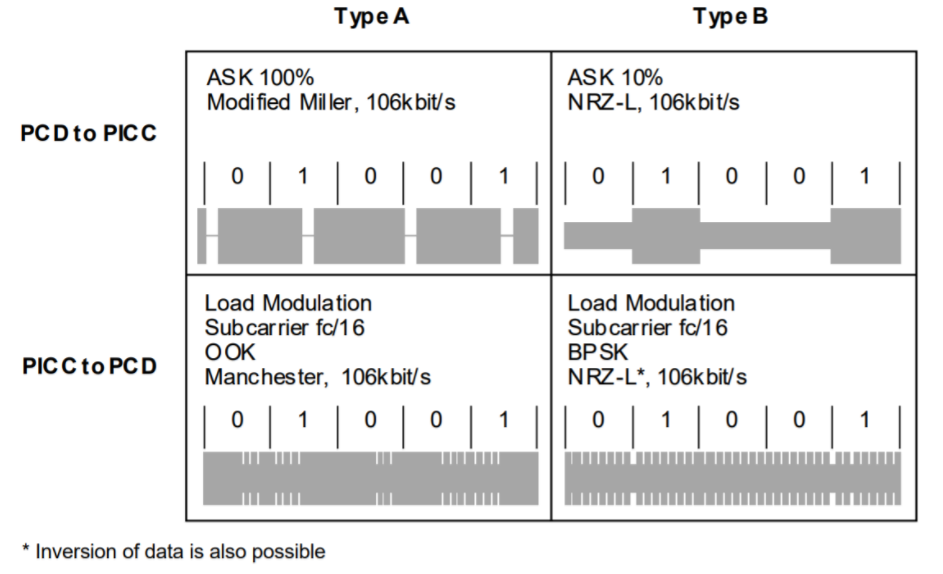
\includegraphics[width=0.9\linewidth]{otros/tipos_iso.png}
\caption{Tipos de inteface ISO/IEC 14443}
\label{fig:tipos_iso}
\end{figure}

\subsubsection{Interfaz de comunicación tipo “A”}

\begin{enumerate}
\item Comunicación PCD a PICC
\begin{itemize}
\item \textbf{Velocidad de transmisión:} durante la inicialización y anticolisión la velocidad de transmisión deberá ser fc/128.
\item \textbf{Modulación:} La comunicación entre el PCD y el PICC se lleva a cabo empleando el principio de modulación ASK 100\% del campo RF para crear la “pausa” como se muestra en la figura \ref{fig:demod_tipoa}.

\begin{figure}[H]
\centering
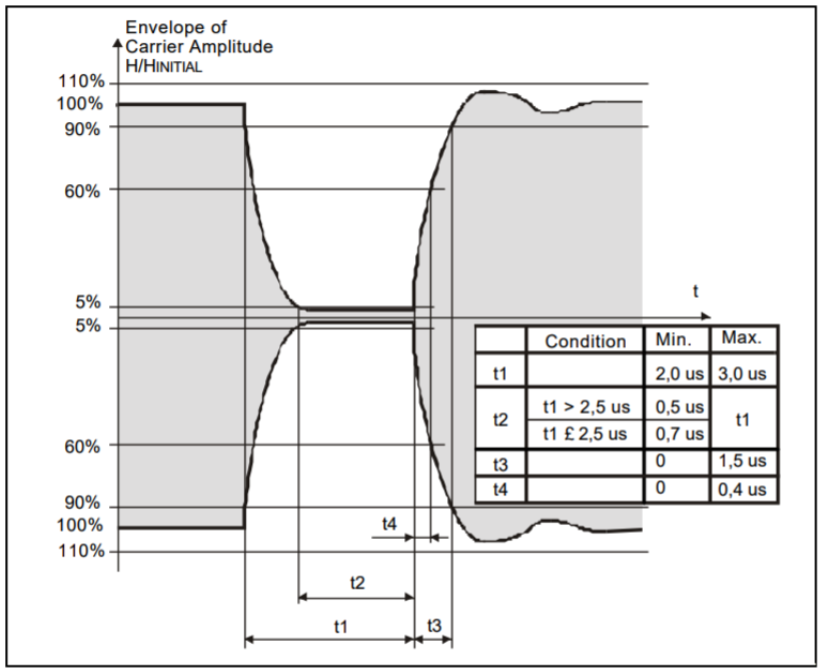
\includegraphics[width=0.7\linewidth]{otros/demod_tipoa.png}
\caption{Modulación PCD a PICC}
\label{fig:demod_tipoa}
\end{figure}

La envolvente del campo del PCD deberá decrementar monótonamente a menos del 5\% de su valor inicial (Hinicial) y permanecer de esta manera por un tiempo mayor a “t2”.

Si la envolvente del campo del PCD no decrementa monótonamente, el tiempo entre un máximo local y el tiempo del paso del mismo valor antes del máximo local no deberá exceder  los 0.5us. Esto solo aplicará si el máximo local es mayor al 5\% del H inicial.

El sobrepaso deberá permanecer entre el 90\% y el 110\% del H inicial.

El PICC deberá detectar el “Fin de pausa” (End of Pause) luego de que el campo exceda el 5\% del H inicial y antes de que supere el 60\% del mismo.

En la figura \ref{fig:pausa_tipoa} se procede a mostrar la definición del “Fin de Pausa” (EoP).

\begin{figure}[H]
\centering
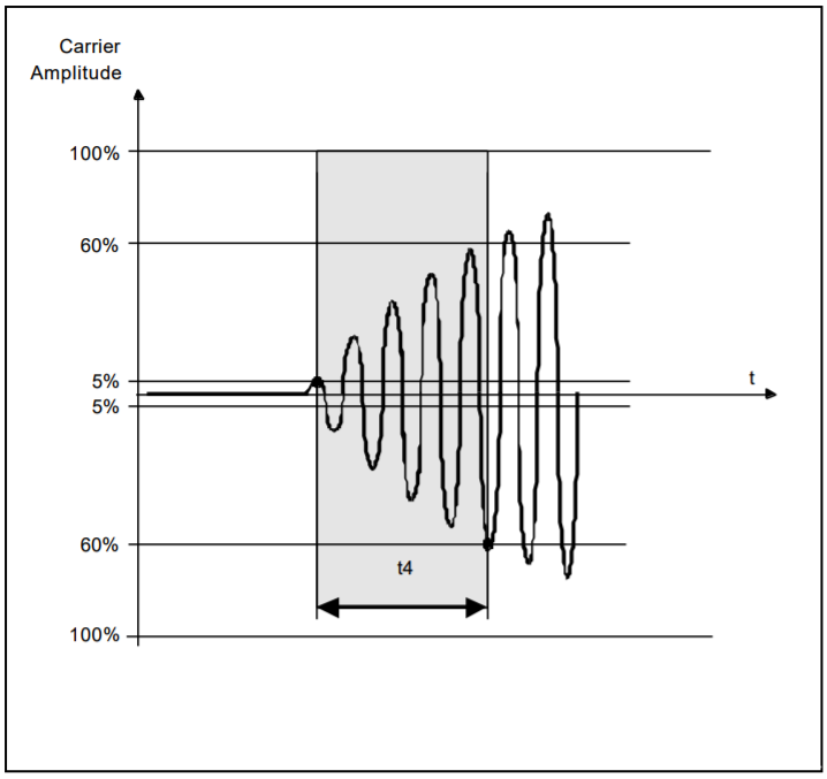
\includegraphics[width=0.7\linewidth]{otros/pausa_tipoa.png}
\caption{Fin de la pausa - ISO/IEC 14443A}
\label{fig:pausa_tipoa}
\end{figure}

\item \textbf{Representación de los bits y codificación:} Las secuencias están definidas en la tabla \ref{fig:code_tipoa} y la codificación en la tabla \ref{fig:dem_cod_tipoa}.

\begin{figure}[H]
\centering
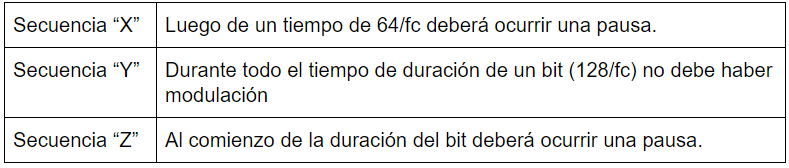
\includegraphics[width=0.9\linewidth]{otros/secuencia_tipoa.png}
\caption{Secuencia PCD a PICC}
\label{fig:code_tipoa}
\end{figure}

\begin{figure}[H]
\centering
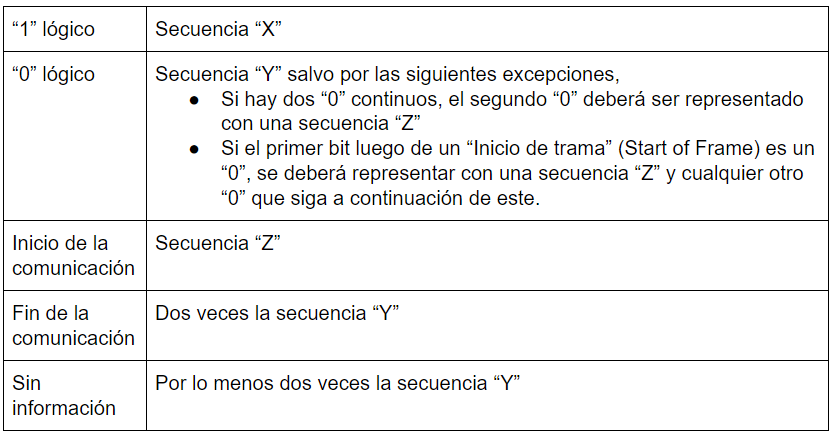
\includegraphics[width=0.9\linewidth]{otros/dem_codigo_tipoa.png}
\caption{Codificación PCD a PICC}
\label{fig:dem_cod_tipoa}
\end{figure}


\end{itemize}

\item Comunicación PICC a PCD

\begin{itemize}
\item \textbf{Velocidad de la información:} Al igual que la comunicación del PCD al PICC, la velocidad durante la inicialización y la anticolisión deberá ser de fc/128 (106 kbit/s).
\item \textbf{Carga de la modulación:} El PICC debera ser capaz de comunicarse hacía el PCD a través del acoplamiento inductivo en donde la frecuencia de la portadora será empleada para generar una subportadora de frecuencia fs. Esta subportadora deberá ser generada empleando una carga en el PICC. La amplitud de la modulación deberá ser por lo menos de 30/H mV, en donde H será el valor RMS de la fuerza del campo magnético en A/m.
\item \textbf{Subportadora:} La frecuencia fs debe ser de fc/16 (847kHz). Consecuentemente con esto, durante la inicialización y la anticolisión, la duración de un bit será equivalente a 8 periodos de la subportadora.
\item \textbf{Modulación de la subportadora:} Cada bit comienza su periodo con una fase definida en relación con la subportadora. El periodo del mismo comienza con el estado cargado de la subportadora. Esta deberá ser modulada usando modulacion on/off con las secuencias definidas en la tabla \ref{fig:mod_cod_tipoa}.

\begin{figure}[H]
\centering
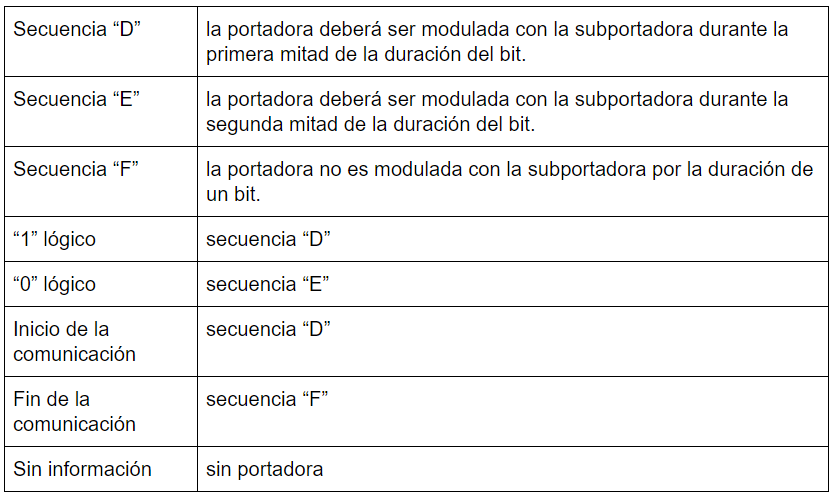
\includegraphics[width=0.9\linewidth]{otros/mod_codigo_tipoa.png}
\caption{Codificación PICC a PCD}
\label{fig:mod_cod_tipoa}
\end{figure}

\end{itemize}


\end{enumerate}

\subsection{Norma ISO/IEC 14443 Parte 3: Inicialización y anticolisión}
\label{sec:Norma14443-3}
%%%%%%%%%%%%%%%%%%%% Document code starts here %%%%%%%%%%%%%%%%%%%%
\subsubsection{Alcance}
Esta parte de la norma describe\par

\begin{itemize}
	\item Sondeo para PICC’s que ingresan al campo de un PCD.\par

	\item El formato de los bytes, tramas y la sincronización empleada durante la fase inicial de la comunicación entre el PCD y el PICC.\par

	\item Contenido del comando inicial REQ y ATQ.\par

	\item Otros parametros requeridos para la inicialización de la comunicación entre los dispositivos.
\end{itemize}\par

\subsubsection{Normativa de referencia}
Las siguientes normas realizan un aporte para constituir un estándar internacional.\par

\begin{itemize}
	\item ISO/IEC 3309: 1993 Intercambio de información entre sistemas de telecomunicaciones. (High Level Data Link Control)\par

	\item ISO/IEC 7816: 1997 Circuitos integrados en tarjetas con contactos.\par

	\item ISO/IEC 14443/2: Circuitos integrados en tarjetas sin contactos - Tarjetas de proximidad.\par

	\item ITU-T Recomendations V.41
\end{itemize}\par

\subsubsection{Términos y definiciones}
Para los propositos de este estándar internacional los términos y definiciones dados en ISO/IEC 14443-2, ISO/IEC 7816-3 y los siguientes aplican.\par

\paragraph{Loop anti-colisión}
Algoritmo empleado para preparar al PCD para dialogar entre una o más PICC’s dentro de su campo energizante.\par


\vspace{\baselineskip}
\paragraph{Protocolo detección de colisión de bits}
Método de anticolisión empleando detección de colisión a nivel de los bits entre tramas. Una colisión ocurre cuando al menos dos PICC’s transmiten patrones complementarios de bits (ver ISO/IEC 14443-2 sección 8.4.2) hacia el PCD. En este caso los patrones de bits son unidos y la portadora es modulada con la subportadora durante toda la duración del bit.\par

El PCD detecta la colisión de bits y reconoce todos los PICC’s en orden de cascada\par


\vspace{\baselineskip}
\paragraph{Byte}
Un byte consta de 8 bits de datos designados b1 a b8, comenzando por el bit más significativo (MSB, b8) hacia el bit menos significativo (LSB, b1).\par


\vspace{\baselineskip}
\paragraph{Colisión}
La transmisión de dos PICC’s en el mismo campo energizante de un PCD y durante el mismo periodo de tiempo, tanto como para que el PCD no logre distinguir el PICC originario de la información.\par


\vspace{\baselineskip}
\paragraph{Unidad Elemental de Tiempo (ETU)}
Para esta parte de la ISO/IEC 14443, un ETU esta definido como\par

\paragraph{Trama (Frame)}
Una trama es una serie de bits de información y, opcionalmente, bits para detección de errores, con delimitadores de trama al inicio y al final de la misma.\par

\paragraph{Capa superior}
Perteneciendo a la aplicación o a capas superiores del protocolo, esto no será descripto en este apartado.\par

\paragraph{Protocolo de intervalo temporal}
Método en donde el PCD establece los canales lógicos con uno o más PICC’s, en el cual se realiza la asignación de los intervalos temporales para la respuesta del PICC.\par

\paragraph{Identificador Único (UID)}
Es un número necesario para el algoritmo de anti-colisión del $``$Tipo A$"$ .\par

\subsubsection{Simbolos (y terminos abreviados)}
Para esta parte de la norma, las abreviaturias utilizadas son:\par

\begin{itemize}
	\item AFI Application Familly Identifie.\par

	\item APa Anticolisión Prefijo a, usado en ATQB\par

	\item APc Anticolisión Prefijo c, usado en Attribute\par

	\item APf Anticolisión Prefijo f, usado en REQB\par

	\item APn Anticolisión Prefijo n, usado en el comando Slot-MARKER\par

	\item ATA Respuesta a ATTRIB\par

	\item ATQ Respuesta a REQUEST\par

	\item ATQA Respuesta a REQUEST del Tipo A\par

	\item ATQB Respuesta a REQUEST del Tipo B\par

	\item ATTRIB Comando de selección del PICC\par

	\item BCC UID CLn checkbyte, calculado como una or exclusivede los 4 bytes anteriores\par

	\item CLn Nivel de cascada\par

	\item CT Tag de cascada, ‘88’\par

	\item CRC\_A Código del ciclo de chequeo redundante de errores definido en 6.1.10\par

	\item CRC\_B Ciclo de chequeo redundante de errores definido en 7.2\par

	\item DESEL Comando para anular la selección\par

	\item E Fin de la comunicación del Tipo A\par

	\item EGT Tiempo de guarda extra (Extra Guard Time)\par

	\item EOF Fin de la trama (End Of Frame), Tipo B\par

	\item ETU Unidad de tiempo elemental, duración de un bit de la transmisión.\par

	\item FGT\ Tiempo de guarda de  la trama (Frame Guard Time)\par

	\item Fc Frecuencia de portadora (13,56 MHz)\par

	\item Fs Frecuencia de la subportadora\par

	\item ID Número de identificación\par

	\item INF Campo de información perteneciente a la capa superior\par

	\item LSB Bit menos significativo (Least Significant Bit)\par

	\item MSB Bit más significativo (Most Significant Bit)\par

	\item N Cantidad de espacios para la anticolisión.\par

	\item NAD Dirección del nodo (Node ADdress)\par

	\item NVB Número de bits validos (Number of Valid Bits)\par

	\item P Bit de paridad impar (Odd parity bit)\par

	\item PARAM Parámetro\par

	\item PCD Dispositivo de acoplamiento de proximidad (Proximity Coupling Device)\par

	\item PICC Tarjeta de proximidad\par

	\item PUPI Identificador Pseudo-Único del PICC\par

	\item REQA Comando de solicitud (Request Command), Tipo A\par

	\item REQB Comando de solicitud (Request Command), Tipo B\par

	\item S Inicio de la comunicación, Tipo A\par

	\item SAK Reconocimiento de SELECT\par

	\item SEL Comando SELECT\par

	\item SOF Inicio de trama $\ast$ Start Of Frame), Tipo B\par

	\item UID Identificador Único (Unique IDentification)\par

	\item UIDn Cantidad de bytes del UID
\end{itemize}\par

\subsubsection{Sondeo}
Cuando un PICC se expone a un campo operativo no modulado (ver ISO / IEC 14443-2), debe poder aceptar una solicitud dentro de los 5 ms.\par

Por ejemplo, \par

Cuando un PICC tipo A recibe cualquier comando de tipo B, debe poder aceptar un REQA dentro de los 5 ms.\par

Cuando un PICC tipo B recibe un comando de tipo A, debe poder aceptar un REQB dentro de los 5 ms.\par

Con el fin de detectar los PICCs que entran en su campo energizante, un PCD envía comandos de Solicitud repetidos y busca un ATQ. Los comandos de solicitud usarán REQA y REQB descritos en este documento en cualquier secuencia y además podrán usar otros codificación (es) descrita (s) en el Anexo C. Este proceso se denomina "Sondeo".\par

\subsubsection{Tipo A - Inicialización y anticolisión}
Esta sección describe el protocolo de detección de colisiones de bits aplicable para los PICC de tipo A.\par

\paragraph{Byte, formato de trama y comando y tiempo.}
Esta sección define los formatos del byte de la trama del comando y el tiempo utilizado durante la inicialización de la comunicación y anticolisión. Para la representación y codificación de bits, consulte ISO / IEC 14443-2.\par

\paragraph{Tiempo de retardo de trama}
El tiempo de retardo de trama (FDT) se define como el tiempo entre dos tramas transmitidas en direcciones opuestas.\par

\paragraph{Tiempo de protección de trama}
El tiempo de protección de trama (FGT) se define como el tiempo de retardo de trama mínimo.\par

\paragraph{Tiempo de retardo de trama PCD a PICC}
Este es el tiempo entre el final de la última pausa transmitida por el PCD y el primer borde de modulación dentro del bit de inicio transmitido por el PICC, deberá respetar el tiempo definido en la figura 6.1, donde n es un valor entero.\par


\vspace{\baselineskip}


%%%%%%%%%%%%%%%%%%%% Figure/Image No: 1 starts here %%%%%%%%%%%%%%%%%%%%

\begin{figure}[H]
	\begin{center}
		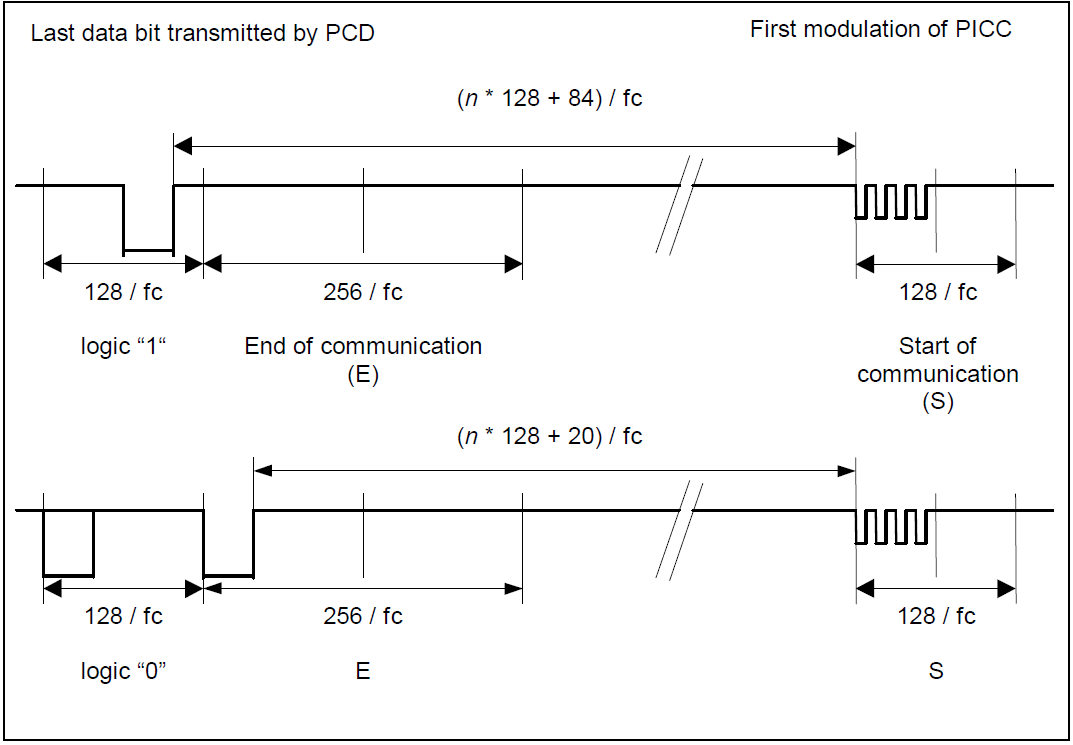
\includegraphics[width=6.1in,height=4.22in]{Norma_ISO/14443-3/media//image9.png}
        \end{center}
\end{figure}


%%%%%%%%%%%%%%%%%%%% Figure/Image No: 1 Ends here %%%%%%%%%%%%%%%%%%%%

\par
\begin{center}
Figura 3.7.6.1 - Demora temporal de trama PCD a PICC.
\end{center}
\par


\paragraph{Tiempo de retardo trama PICC a PCD}
Este es el tiempo transcurrido entre la última modulación transmitida por el PICC y la primera pausa transmitida por el PCD y deberá ser al menos 1172 / fc.\par

\paragraph{Tiempo de guardia de solicitud}
El Tiempo de guardia de solicitud se define como el tiempo mínimo entre los bits de inicio de dos comandos REQUEST consecutivos. Eso tiene el valor 7000 / fc.\par

\paragraph{Formatos de trama}
Los siguientes tipos de tramas se definen para el protocolo de detección de colisiones de bits.\par

\paragraph{Tramas REQA y WAKE-UP}
Las tramas de solicitud (REQA) y activación (WAKE-UP) se utilizan para iniciar la comunicación y consisten en, en el siguiente orden:\par

\begin{itemize}
	\item Inicio de comunicación\par

	\item 7 bits de datos transmitidos LSB primero. (El contenido de los datos es '26' para un REQA estándar y '52' para una solicitud de WAKE-UP).\par

	\item Fin de la comunicación
\end{itemize}\par

No se agrega bit de paridad.\par

%%%%%%%%%%%%%%%%%%%% Figure/Image No: 2 starts here %%%%%%%%%%%%%%%%%%%%
\begin{figure}[H]
	\begin{center}
		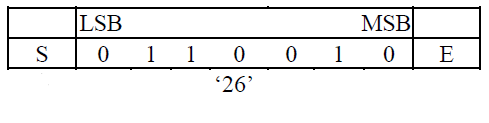
\includegraphics[width=3.76in,height=0.95in]{Norma_ISO/14443-3/media/image6.png}
        \end{center}
\end{figure}
%%%%%%%%%%%%%%%%%%%% Figure/Image No: 2 Ends here %%%%%%%%%%%%%%%%%%%%

\par
\begin{center}
Figura 3.7.6.2 -Tramas REQA y WAKE-UP.
\end{center}
\par

\par
\paragraph{Trama estándar}
Las tramas estándar se utilizan para el intercambio de datos y consisten en,\par

\begin{itemize}
	\item Inicio de comunicación\par

	\item N $\ast$  (8 bits de datos + bit de paridad impar). El LSB de cada byte de datos se transmite primero. Cada byte de datos es seguido por un bit de paridad impar.\par

	\item Fin de la comunicación
\end{itemize}\par

\paragraph{Marco de anticolisión orientado a bits}
Se detecta una colisión cuando al menos dos PICC transmiten patrones de bits diferentes a la PCD. En este caso, la portadora se modula con la subportadora durante toda la duración del bit para al menos un bit.\par

Las tramas de anticolisión orientadas a bits solo se utilizan durante los ciclos anticolisión de tramas de bits y son, de hecho, tramas estándar con una longitud de 7 bytes de datos, divididos en dos partes: parte 1 para transmisión de PCD a PICC y parte 2 para transmisión desde PICC a PCD.\par

Para la duración de la parte 1 y parte 2, se aplicarán las siguientes reglas:\par

Regla 1: La suma de los bits de datos será 56\par

Regla 2: la longitud mínima de la parte 1 será de 16 bits de datos\par

Regla 3: la longitud máxima de la parte 1 será de 55 bits de datos\par

En consecuencia, la longitud mínima de la parte 2 será de 1 bit de datos y la longitud máxima será de 40 bits de datos.\par

Como la división puede ocurrir en cualquier posición de bit dentro de un byte de datos, se definen dos casos:\par

Caso FULL BYTE: división después de un byte de datos completo. Se agrega un bit de paridad después del último bit de datos de la parte 1.\par

Caso SPLIT BYTE: división dentro de un byte de datos. No se agrega ningún bit de paridad después del último bit de datos de part1.\par

\paragraph{CRC\_A}
El proceso de codificación y verificación CRC\_A se define en la recomendación UIT-T V.41, párrafo 2. El polinomio generador utilizado para generar los bits de verificación es x $ \string^ $  16 + x $ \string^ $  12 + x $ \string^ $  5 + 1. El valor inicial será ' 6363 '. El CRC\_A se adjuntará a los bytes de datos y se transmitirá a través de tramas estándar.\par

\paragraph{Estados del PICC.}
Las siguientes secciones proporcionan descripciones de los estados para un PICC de tipo A específico del protocolo de detección de colisiones de bits.\par



%%%%%%%%%%%%%%%%%%%% Figure/Image No: 3 starts here %%%%%%%%%%%%%%%%%%%%

\begin{figure}[H]
	\begin{center}
		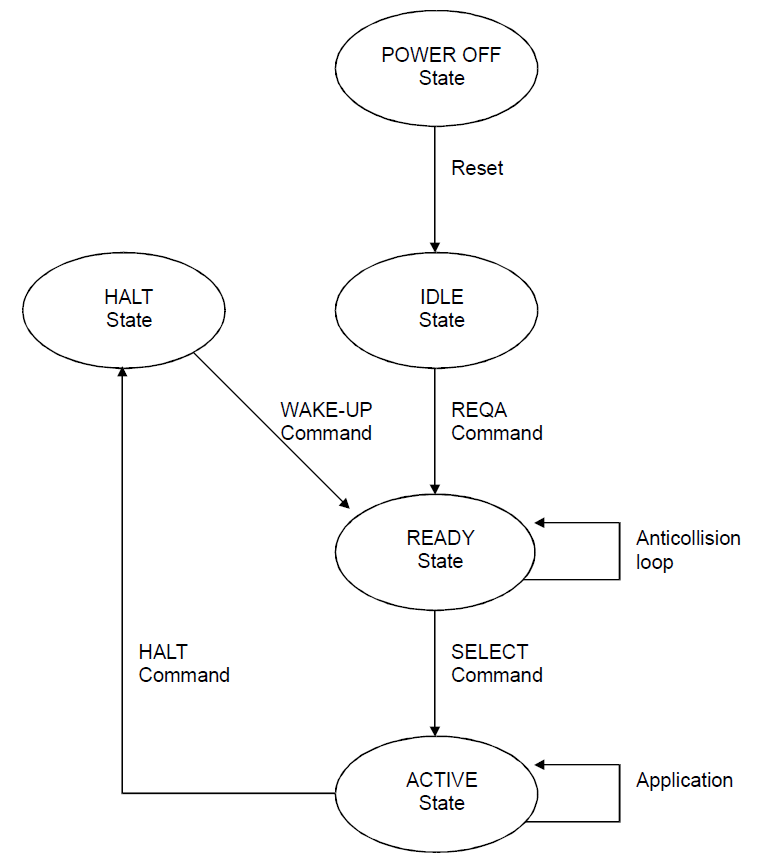
\includegraphics[width=6.27in,height=7.01in]{Norma_ISO/14443-3/media/image7.png}
        \end{center}
\end{figure}


%%%%%%%%%%%%%%%%%%%% Figure/Image No: 3 Ends here %%%%%%%%%%%%%%%%%%%%

\par

\par
\begin{center}
Figura 3.7.6.3 - Diagrama de estados PICC Tipo $``$A$"$ 
\end{center}
\par

\paragraph{Estado OFF}
En el estado de OFF, el PICC no recibe energía debido a la falta de energía del portador y no debe emitir subportadora.\par

\paragraph{Estado IDLE}
Después de que el campo haya estado activo durante un retraso máximo definido en la cláusula 5, el PICC ingresará en su estado IDLE. En este estado, el PICC está encendido, y es capaz de demodular y reconocer los comandos válidos de REQA y WAKE-UP del PCD.\par

\paragraph{Estado READY}
Este estado se ingresa tan pronto como se recibe y sale un mensaje REQA o WAKE-UP válido cuando el PICC está seleccionado con su UID. En este estado, se puede aplicar la anticolisión de la trama de bits u otro método anticolisión opcional. Los niveles de cascada se manejan dentro de este estado para obtener todo el UID CLn.\par

\paragraph{Estado ACTIVE}
Este estado se ingresa seleccionando el PICC con su UID completo.\par

\paragraph{Estado HALT}
Este estado se ingresa mediante el comando HALT definido en 3.7.6.3.4 o mediante un comando específico de la aplicación no definido en esta parte de ISO / IEC 14443. En este estado, un PICC responderá solo a un comando de WAKE-UP, que transita el PICC a su estado READY.\par

\paragraph{Conjunto de comandos}
Los comandos utilizados por el PCD para gestionar la comunicación con varios PICC son:\par

\begin{itemize}
	\item REQA\par

	\item WAKE-UP\par

	\item ANTICOLLISION\par

	\item SELECT\par

	\item HALT
\end{itemize}\par

Los comandos usan los formatos de byte y marco descriptos anteriormente.\par

\paragraph{Comando REQA}
El comando REQA es enviado por el PCD para sondear el campo de los PICC de tipo A.\par

\paragraph{Comando WAKE-UP}
El PCD envía el comando WAKE-UP para poner los PICC que han ingresado al estado HALT de nuevo en el estado READY. Luego, participarán en nuevos procedimientos de anticolisión y selección.\par

\paragraph{Comandos ANTICOLLISION y SELECT}
Estos comandos se usan durante un ciclo anticolisión. Los comandos ANTICOLLISION y SELECT constan de:\par

\begin{itemize}
	\item Seleccionar código SEL (1 byte)\par

	\item Número de bits válidos NVB (1 byte)\par

	\item De 0 a 40 bits de datos de UID CLn según el valor de NVB
\end{itemize}\par

SEL especifica el nivel de cascada CLn.\par

NVB especifica el número de bits válidos de UID CLn transmitidos por el PCD.\par

\paragraph{Comando HALT}
El comando HALT consta de cuatro bytes y se transmitirá utilizando la trama estándar.\par



%%%%%%%%%%%%%%%%%%%% Figure/Image No: 4 starts here %%%%%%%%%%%%%%%%%%%%

\begin{figure}[H]
	\begin{center}
		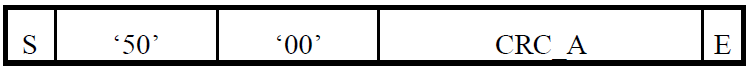
\includegraphics[width=5.47in,height=0.51in]{Norma_ISO/14443-3/media/image10.png}
        \end{center}
\end{figure}


%%%%%%%%%%%%%%%%%%%% Figure/Image No: 4 Ends here %%%%%%%%%%%%%%%%%%%%

\par
\begin{center}
Figura 3.7.6.4 - Trama del comando HALT.
\end{center}
\par

Si el PICC responde con cualquier modulación durante un período de 1 ms después del final de la trama HALT, esta respuesta se interpretará como "no reconocido".\par

\paragraph{Secuencia SELECT}
El propósito de esta secuencia es el de obtener el UID de un PICC y seleccionar a este PICC para una futura comunicación.\par

\paragraph{ATQA - Respuesta al comando REQA}
Después de que el PCD transmite el comando REQA, todos los PICC responden de forma síncrona con su respuesta (ATQA), que codifica el tipo anticolisión aplicable en dos bytes de datos.\par

Si hay múltiples respuestas PICC, pueden producirse colisiones. El PCD decodificará una colisión dentro de ATQA. Esto da como resultado un OR lógico de todos los ATQA.\par

\paragraph{Anticolisión y selección}
\paragraph{Bucle anticolisión dentro de cada nivel de cascada}
El siguiente algoritmo se aplicará al ciclo anticolisión:\par

\begin{itemize}
	\item Paso 1: El PCD asigna SEL con el código para el tipo de anticolisión seleccionado y el nivel de cascada.\par

	\item Paso 2: El PCD asigna NVB con el valor de '20'.\par

	\item Paso 3: El PCD transmite SEL y NVB.\par

	\item Paso 4: Todos los PICC en el campo responderán con su UID CLn completa.\par

	\item Paso 5: Suponiendo que los PICC en el campo tengan números de serie únicos, entonces, si responde más de un PICC, se produce una colisión. Si no ocurre una colisión, se omiten los pasos 6 a 10.\par

	\item Paso 6: El PCD reconocerá la posición de la primera colisión.\par

	\item Paso 7: El PCD asigna NVB con un valor que especifica el número de bits válidos de UID CLn. Los bits válidos serán parte del UID CLn que se recibió antes de que ocurriera una colisión añadida por un (0) by (1) b, decidido por el PCD. Una implementación típica agrega a (1) b.\par

	\item Paso 8: El PCD transmite SEL y NVB, seguidos de los bits válidos.\par

	\item Paso 9: Solo los PICC cuya parte de UID CLn es igual a los bits válidos transmitidos por el PCD transmitirán sus bits restantes del UID CLn.\par

	\item Paso 10: Si ocurren más colisiones, se repiten los pasos 6 a 9. La cantidad máxima de bucles será 32.\par

	\item Paso 11: Si no hay más colisiones, la PCD asigna NVB con el valor de '70'.\par

	\item Paso 12: El PCD transmite SEL y NVB, seguidos de los 40 bits de UID CLn, seguidos por CRC\_A suma de comprobación.\par

	\item Paso 13: El PICC que UID CLn coincide con los 40 bits responde con su SAK.\par

	\item Paso 14: Si el UID está completo, el PICC transmitirá SAK con un bit en cascada despejado y el tránsito desde el estado LISTO al estado ACTIVO.\par

	\item Paso 15: El PCD verificará si el bit en cascada de SAK está configurado para decidir si seguirán ciclos de anticolisión adicionales con un nivel de cascada incrementado.
\end{itemize}\par

Si el UID de un PICC es conocido, el PCD puede omitir el paso 2 al paso 10 para seleccionar este PICC sin realizar el ciclo anticolisión.\par

\paragraph{Código de SEL}
Longitud: 1 byte\par

Valores posibles: '93', '95', '97'.\par

\paragraph{Código de NVB (número de bits válidos)}
Longitud: 1 byte\par

Los 4 bits superiores se llaman por cuenta y especifican el número de todos los bits de datos válidos divididos entre 8, incluidos SEL y NVB transmitidos por el PCD. En consecuencia, el valor mínimo de bytecount es 2 y el valor máximo es 7.\par

Los 4 bits más bajos se denominan bitcount y especifican el número de todos los bits de datos válidos módulo 8 transmitidos por el PCD.\par

\paragraph{Código de SAK}
SAK es transmitido por el PICC cuando NVB ha especificado 40 bits de datos válidos y cuando todos estos bits de datos coinciden con UID CLn.\par

SAK se transmite a través la trama estándar, seguido de CRC\_A.\par

Si el UID no está completo, el PICC permanecerá en estado READY y el PCD iniciará un nuevo ciclo de anticolisión con un nivel de cascada incrementado.\par

Si el UID está completo, el PICC transmitirá SAK con el bit de cascada despejado y el tránsito del estado READY al estado ACTIVE. El PICC configurará el bit b6 de SAK cuando haya información adicional disponible.\par

La definición de la información adicional no está sujeta a esta parte del estándar y se definirá en ISO / IEC 14443-4.\par

\paragraph{Contenido de UID y niveles de cascada}
El UID consta de 4, 7 o 10 bytes UID. En consecuencia, el PICC manejará hasta 3 niveles de cascada para obtener todos los bytes de UID.\par

Dentro de cada nivel de cascada, una parte del UID que consta de 5 bytes de datos se transmitirá a la PCD. De acuerdo con la nivel de cascada máximo, se definen tres tipos de tamaño de UID. Este tamaño de UID debe ser consistente con la tabla 6.4.\par



%%%%%%%%%%%%%%%%%%%% Figure/Image No: 5 starts here %%%%%%%%%%%%%%%%%%%%

\begin{figure}[H]
	\begin{center}
		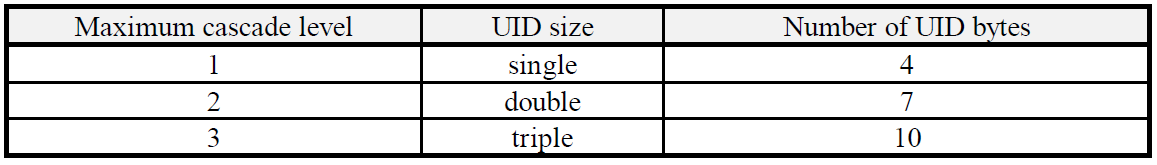
\includegraphics[width=6.27in,height=0.89in]{Norma_ISO/14443-3/media/image8.png}
        \end{center}
\end{figure}


%%%%%%%%%%%%%%%%%%%% Figure/Image No: 5 Ends here %%%%%%%%%%%%%%%%%%%%

\par
\begin{center}
Figura 3.7.6.4 - Tamaños de los UID.
\end{center}
\par

\subsection{Norma ISO/IEC 14443 Parte 4: Protocolo de transmisión}
\label{sec:Norma14443-4}
%%%%%%%%%%%%%%%%%%%% Document code starts here %%%%%%%%%%%%%%%%%%%%
\subsubsection{Alcance}
Esta parte de ISO / IEC 14443 especifica un protocolo de transmisión de bloques semidúplex que presenta las necesidades especiales de un entorno sin contacto y define la secuencia de activación y desactivación del protocolo.\par

Esta parte de ISO / IEC 14443 se utilizará junto con otras partes de ISO / IEC 14443 y se aplica a las tarjetas de proximidad de tipo A y tipo B.\par

\subsubsection{Referencias normativas}
Las siguientes normas contienen disposiciones que, a través de la referencia en este texto, constituyen disposiciones de esta parte de ISO / IEC 14443. En el momento de la publicación, las ediciones indicadas eran válidas. Todos los estándares están sujetos a revisión,\par

y se alienta a las partes de los acuerdos basados ​​en esta parte de ISO / IEC 14443 a investigar la posibilidad de aplicar las normas Internacionales válidas más recientes.\par

ISO / IEC 7816-3, Tarjetas de identificación - Tarjetas de circuito (s) integrado (s) con contactos - Parte 3: señales electrónicas y protocolos de transmisión.\par

ISO / IEC 7816-4, Tarjetas de identificación - Tarjetas de circuito (s) integrado (s) con contactos - Parte 4: Comandos interindustriales para el intercambio.\par

\subsubsection{Término (s) y definición (es)}
\paragraph{Duración del bit.}
La duración del bit se define como una unidad de tiempo elemental (ETU). El ETU se calcula con la siguiente fórmula:\par

1 etu = 128 / (D x fc)\par

El valor inicial del divisor D será 1.\par

La frecuencia portadora fc se define en ISO / IEC 14443-2.\par

\paragraph{Bloque.}
Un tipo especial de trama, que contiene un formato de datos de protocolo válido. Un formato de datos de protocolo válido incluye I-blocks, R-blocks o S-blocks.\par

\paragraph{Bloque inválido.}
Un tipo de trama, que contiene un formato de protocolo no válido. Un tiempo de espera, cuando no se ha recibido ningún marco, no es interpretado como un bloque inválido.\par

\paragraph{Trama}
Como se define en ISO / IEC 14443-3. El PICC tipo A usa la trama estándar definido para el tipo A y el PICC tipo B usa la trama definido para el tipo B.\par


\vspace{\baselineskip}
\subsubsection{Símbolos (y términos abreviados)}
\begin{itemize}
	\item ACK - Reconocimiento positivo\par

	\item ATS - Respuesta a SELECT\par

	\item ATQB - Respuesta a la búsqueda de PICC tipo B\par

	\item CID - IDentificador de tarjeta\par

	\item CRC - Comprobación de redundancia cíclica, como se define para cada tipo de PICC en ISO / IEC 14443-3\par

	\item D - Divisor\par

	\item DR - Divisor recibido (PCD a PICC)\par

	\item DS - Divisor enviado (PICC a PCD)\par

	\item EDC - Código de detección de errores\par

	\item ETU - Unidad de tiempo elemental\par

	\item fc - Frecuencia portadora\par

	\item FSC - Tamaño de la trama para la tarjeta de proximidad\par

	\item FSD - Tamaño de la trama para el dispositivo de acoplamiento de proximidad\par

	\item FWT - Tiempo de espera de tramas\par

	\item FWTTEMP - Tiempo de espera temporal de trama\par

	\item HLTA - Comando HALT para PICC tipo A\par

	\item I-block - Bloque de información\par

	\item INF - Campo de información\par

	\item NAD - Nodo de dirección\par

	\item NAK - No reconocido\par

	\item OSI - Interconexión de sistemas abiertos\par

	\item PCB -Byte de control de protocolo\par

	\item PCD - Dispositivo de acoplamiento de proximidad\par

	\item PICC - Tarjeta de proximidad\par

	\item PPS - Protocolo y selección de parámetros\par

	\item PPSS - Inicio de protocolos y selección de parámetros\par

	\item PPS0 - Protocolo y selección de parámetros 0\par

	\item PPS1 - Protocolo y selección de parámetros 1\par

	\item R-block - Bloque READY recibido\par

	\item R (ACK) - R-block que contiene un reconocimiento positivo\par

	\item R (NAK) - R-block que contiene un reconocimiento negativo\par

	\item RATS - Solicitud de respuesta para SELECT\par

	\item RFU - Reservado para uso futuro\par

	\item S-block - Bloque de supervisión\par

	\item SAK - Reconocimiento de SELECT\par

	\item SFGT - Tiempo de protección de inicio de trama\par

	\item WUPA - Comando Wake-Up para PICC tipo A\par

	\item WTX - Extensión del tiempo de espera\par

	\item WTXM - Multiplicador de la extensión de tiempo de espera
\end{itemize}\par

\paragraph{Activación de protocolo de PICC tipo A}
Se aplicará la siguiente secuencia de activación: \par

\begin{itemize}
	\item Secuencia de activación de PICC como se define en ISO / IEC 14443-3 (petición, ciclo anticolisión y selección).\par

	\item Al principio, se debe verificar el byte SAK para determinar la disponibilidad de un ATS. El SAK se define en ISO / IEC 14443-3.\par

	\item El PICC puede configurarse en estado HALT, usando el comando HLTA como se define en ISO / IEC 14443-3, si no hay ATS disponible.\par

	\item El PCD puede enviar el RATS como siguiente comando después de recibir el SAK si hay un ATS disponible.\par

	\item El PICC enviará su ATS como respuesta a las RATS. El PICC solo responderá a las RATS si la RATS es recibido directamente después de la selección.\par

	\item Si el PICC admite cualquier parámetro modificable en el ATS, el PCD puede utilizar una solicitud de PPS como siguiente comando después de recibir el ATS para cambiar los parámetros.\par

	\item El PICC enviará una respuesta de PPS como respuesta a la solicitud de PPS.
\end{itemize}\par

Un PICC no necesita implementar el PPS, si no admite ningún parámetro modificable en el ATS.\par



%%%%%%%%%%%%%%%%%%%% Figure/Image No: 1 starts here %%%%%%%%%%%%%%%%%%%%

\begin{figure}[H]
	\begin{center}
		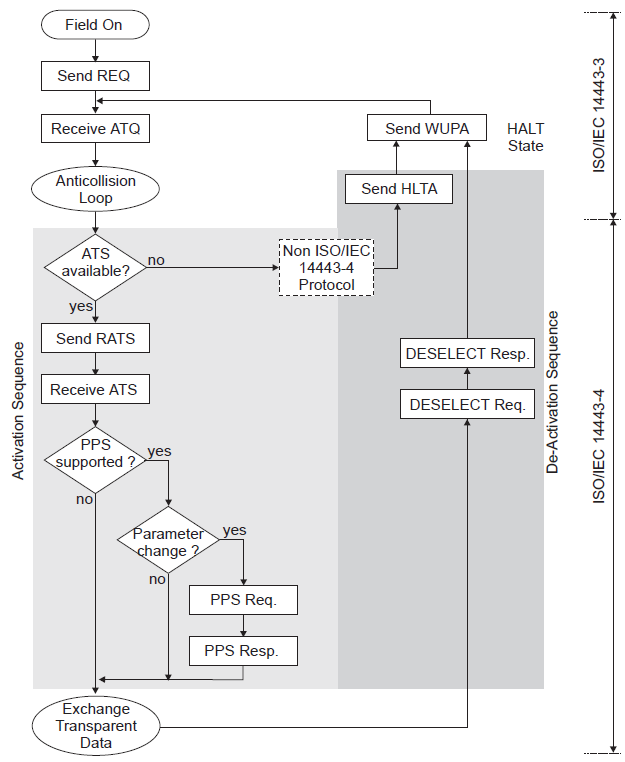
\includegraphics[width=6.27in,height=7.64in]{Norma_ISO/14443-4/media/image8.png}
    \end{center}
\end{figure}


%%%%%%%%%%%%%%%%%%%% Figure/Image No: 1 Ends here %%%%%%%%%%%%%%%%%%%%

\par
\begin{center}
\textbf{Figura 3.8.5.1 - Activación de un PICC Tipo A desde un PCD}
\end{center}
\par

\paragraph{Solicitud de respuesta para seleccionar}
Esta cláusula define las RATS con todos sus campos\par

El byte de parámetro consta de dos partes (figura 3.8.5.2):\par

El medio byte b8 a b5 más significativo se denomina FSDI y codifica FSD. El FSD define el tamaño máximo de una trama que el PCD puede recibir.\par

El medio byte menos significativo b4 a b1 se denomina CID y define el número lógico del PICC direccionado en el rango de 0 a 14. El valor 15 es RFU. El CID está especificado por el PCD y será único para todos PICCs, que están en el estado ACTIVO al mismo tiempo. El CID se fija por el tiempo que el PICC está activo y el PICC usará el CID como su identificador lógico, que está contenido en el primer RATS sin errores recibido.\par


\vspace{\baselineskip}


%%%%%%%%%%%%%%%%%%%% Figure/Image No: 2 starts here %%%%%%%%%%%%%%%%%%%%

\begin{figure}[H]
	\begin{center}
		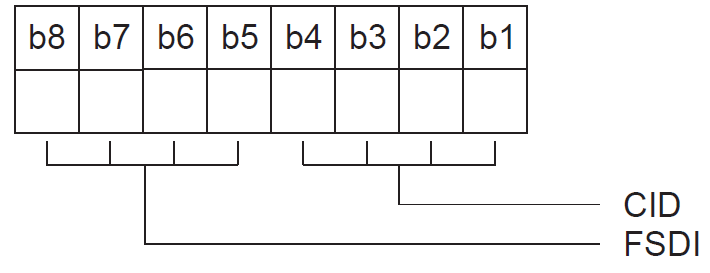
\includegraphics[width=3.84in,height=1.48in]{Norma_ISO/14443-4/media/image5.png}
    \end{center}
\end{figure}


%%%%%%%%%%%%%%%%%%%% Figure/Image No: 2 Ends here %%%%%%%%%%%%%%%%%%%%

\par
\begin{center}
\textbf{Figura 3.8.5.2 - Byte de parámetros del comando RATS.}
\end{center}
\par

\paragraph{Respuesta a SELECT}
Esta cláusula define el ATS con todos sus campos disponibles (Figura 3.8.5.3).\par

En el caso de que uno de los campos definidos no esté presente en un ATS enviado por un PICC, se aplicarán los valores predeterminados para ese campo.\par


\vspace{\baselineskip}


%%%%%%%%%%%%%%%%%%%% Figure/Image No: 3 starts here %%%%%%%%%%%%%%%%%%%%

\begin{figure}[H]
	\begin{center}
		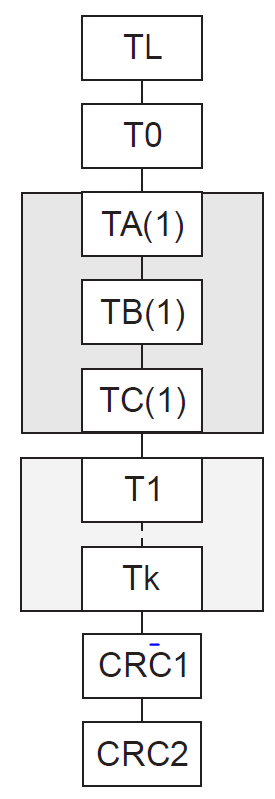
\includegraphics[width=0.88in,height=2.56in]{Norma_ISO/14443-4/media/image3.png}
    \end{center}
\end{figure}


%%%%%%%%%%%%%%%%%%%% Figure/Image No: 3 Ends here %%%%%%%%%%%%%%%%%%%%

\par

\begin{center}
\textbf{Figura 3.8.5.3 - Estructura del comando ATS.}
\end{center}
\par

\paragraph{Estructura de los bytes}
El byte de longitud TL viene seguido de un número variable de bytes posteriores opcionales en el siguiente orden:\par

\begin{itemize}
	\item formato de bytes T0,\par

	\item bytes de interfaz TA (1), TB (1), TC (1) y bytes históricos T1 a Tk.
\end{itemize}\par

\paragraph{Longitud de bytes}
El TL de longitud de bytes es obligatorio y especifica la longitud del ATS transmitido incluido él mismo. Los dos bytes CRC no están incluidos en TL. El tamaño máximo del ATS no debe exceder el FSD indicado. Por lo tanto, el valor máximo de TL no debe exceder el FSD-2.\par

\paragraph{Formato de byte}
El byte de formato T0 es opcional y está presente tan pronto como la longitud sea mayor que 1. El ATS solo puede contener los siguientes bytes opcionales, cuando este byte de formato está presente.\par

T0 consta de tres partes:\par

\begin{itemize}
	\item El bit más significativo b8 se establecerá en 0. El valor 1 es RFU.\par

	\item Los bits b7 a b5 indican la presencia de bytes de interfaz posteriores TA (1), TB (1) y TC (1).\par

	\item El medio byte menos significativo b4 a b1 se llama FSCI y codifica FSC. El FSC define el tamaño máximo de un marco aceptado por el PICC. El valor predeterminado de FSCI es 2 y conduce a un FSC de 32 bytes. La codificación de FSC es igual a la codificación de FSD.
\end{itemize}\par

\paragraph{Byte de interfaz TA (1)}
El byte de interfaz TA (1) consta de cuatro partes:\par

\begin{itemize}
	\item El bit más significativo b8 codifica la posibilidad de manejar diferentes divisores para cada dirección. Cuando este bit se establece en 1, el PICC no puede manejar diferentes divisores para cada dirección.\par

	\item Los bits b7 a b5 codifican la capacidad de tasa de bits del PICC para la dirección de PICC a PCD, llamada DS. El valor predeterminado será (000) b.\par

	\item El bit b4 se establece en (0) b y el otro valor es RFU.\par

	\item Los bits b3 a b1 codifican la capacidad de velocidad de bits del PICC para la dirección de PCD a PICC, llamada DR. El valor predeterminado será (000) b.
\end{itemize}\par

\paragraph{Byte de interfaz TB (1)}
El\ byte de interfaz TB (1) transmite información para definir el tiempo de espera de la trama y el tiempo de guarda  de la trama de inicio.\par

El byte de interfaz TB (1) consta de dos partes:\par

\begin{itemize}
	\item El medio byte b8 a b5 más significativo se denomina FWI y codifica FWT\par

	\item El medio byte menos significativo b4 a b1 se llama SFGI y codifica un valor multiplicador utilizado para definir el SFGT. El SFGT define un tiempo de protección específico que necesita el PICC antes de estar listo para recibir el siguiente cuadro después de haber enviado el ATS. SFG está codificado en el rango de 0 a 14. El valor de 15 es RFU. El valor de 0 indica que no se necesita SFGT y los valores en el rango de 1 a 14 se usan para calcular el SFGT con la fórmula que se indica a continuación. El valor predeterminado de SFG es 0.
\end{itemize}\par

\begin{center}
 \( SFGT= \left( 256\ast\frac{16}{fc} \right) \ast2^{SFG} \) 
\end{center}
\par

\paragraph{Bytes históricos}
Los bytes históricos T1 a Tk son opcionales y aportan información general. La longitud máxima de ATS da la cantidad máxima posible de bytes históricos. ISO / IEC 7816-4 especifica el contenido de los bytes históricos.\par

\paragraph{Petición de selección de protocolo y parámetro}
La solicitud de PPS contiene el byte de inicio seguido de un byte de formato y un byte de parámetro (figura 3.8.5.4).\par


\vspace{\baselineskip}


%%%%%%%%%%%%%%%%%%%% Figure/Image No: 4 starts here %%%%%%%%%%%%%%%%%%%%

\begin{figure}[H]
	\begin{center}
		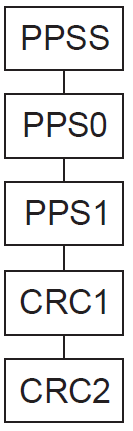
\includegraphics[width=0.53in,height=1.7in]{Norma_ISO/14443-4/media/image7.png}
    \end{center}
\end{figure}


%%%%%%%%%%%%%%%%%%%% Figure/Image No: 4 Ends here %%%%%%%%%%%%%%%%%%%%

\par
\begin{center}
\textbf{Figura 3.8.5.4 - Solicitud de selección de protocolo y parametros.}
\end{center}
\par

\paragraph{Inicio de selección de protocolo y parámetros}
El PPSS consta de dos partes:\par

\begin{itemize}
	\item El medio byte más significativo b8 a b5 es igual a 'D' e identifica el PPS.\par

	\item El medio byte menos significativo b4 a b1 se denomina CID y define el número lógico del PICC direccionado.
\end{itemize}\par

\paragraph{Selección 0 de protocolo y parámetros.}
El PPS0 consta de cuatro partes:\par

\begin{itemize}
	\item b8 a b6 deberá establecerse en (000)b, todos los demás valores son RFU\par

	\item b5 si el PPS1 es transmitido se establece en (1)b.\par

	\item b4 a b2 deberá establecerse en (000)b, todos los demás valores son RFU\par

	\item b1deberá establecerse en (1)b, (0)b es RFU
\end{itemize}\par

\paragraph{Selección 1 de protocolo y parámetros.}
El PPS1 consta de tres partes:\par

\begin{itemize}
	\item El medio byte más significativo b8 a b5 es (0000) b y todos los demás valores son RFU.\par

	\item Los bits b4, b3 se llaman DSI y codifican el divisor entero seleccionado de PICC a PCD.\par

	\item Los bits b2, b1 se llaman DRI y codifican el divisor entero seleccionado de PCD a PICC.
\end{itemize}\par

\paragraph{Respuesta de selección de protocolo y parámetros}
La respuesta de PPS confirma la solicitud de PPS recibida.\par

\paragraph{Tiempo de espera de la trama de activación}
El tiempo de espera de la trama de activación define el tiempo máximo para que un PICC comience a enviar su trama de respuesta después del final de una trama recibida del PCD y tiene un valor de 65536 / fc ($ \sim $  4833 $ \mu $ s).\par

\paragraph{Detección y recuperación de errores}
\paragraph{Manejo de RATS y ATS}
\paragraph{Reglas de PCD}
Cuando el PCD ha enviado el RATS y recibe un ATS válido, el PCD continuará funcionando.\par

En cualquier otro caso, el PCD puede retransmitir la RATS antes de que utilice la secuencia de desactivación tal como se define en la cláusula 8.\par

\paragraph{Reglas del PICC}
Cuando el PICC ha sido seleccionado con el último comando y\par

\begin{enumerate}
	\item Recibe un RATS válido, el PICC deberá\par

\begin{itemize}
	\item enviar de vuelta su ATS y\par

	\item deshabilitar las RATAS (no responda más a las RATS recibidas).
\end{itemize}\par

	\item Recibe cualquier otro bloque válido o inválido, excepto un comando HLTA, el PICC deberá
\end{enumerate}\par

\begin{itemize}
	\item ignorar el bloque y permanezca en modo de recepción.
\end{itemize}\par

\paragraph{Tratamiento de solicitud PPS y respuesta PPS}
\paragraph{Reglas del PCD}
Cuando el PCD ha enviado una solicitud de PPS y recibió una respuesta de PPS válida, el PCD activará los parámetros seleccionados y continuará la operación.\par

En cualquier otro caso, el PCD puede retransmitir una solicitud de PPS y continuar la operación.\par

\paragraph{Reglas de PICC }
Cuando el PICC ha recibido un RATS, envía su ATS y\par

\begin{enumerate}
	\item 1. recibió una solicitud de PPS válida, el PICC deberá\par

\begin{itemize}
	\item envía la respuesta de PPS,\par

	\item deshabilitar la solicitud de PPS (ya no responde a las solicitudes de PPS recibidas) y\par

	\item activar el parámetro recibido.
\end{itemize}\par

	\item Recibió un bloque inválido, el PICC deberá\par

\begin{itemize}
	\item deshabilitar la solicitud de PPS (ya no responde a las solicitudes de PPS recibidas) y\par

	\item permanecer en modo de recepción.
\end{itemize}\par

	\item Recibió un bloque válido, excepto una solicitud de PPS, el PICC deberá
\end{enumerate}\par

\begin{itemize}
	\item deshabilitar la solicitud de PPS (ya no responde a las solicitudes de PPS recibidas) ycontinuar operando
\end{itemize}\par

\paragraph{Manejo del CID durante la activación}
Cuando el PCD ha enviado un RATS que contiene un CID = n distinto a 0 y\par

\begin{enumerate}
	\item Recibió un ATS que indica que el CID es compatible, el PCD deberá\par

\begin{itemize}
	\item enviar bloques que contengan CID = n a este PICC\par

	\item no usar el CID = n para RATS adicionales mientras este PICC esté en estado ACTIVE.
\end{itemize}\par

	\item Recibió un ATS que indica que el CID no es compatible, el PCD deberá enviar bloques que no contengan CID a este PICC y no activar ningún otro PICC mientras este PICC esté en estado ACTIVE.
\end{enumerate}\par

Cuando el PCD ha enviado un RATS que contiene un CID igual a 0 y\par

\begin{enumerate}
	\item Recibió un ATS que indica que CID es compatible, el PCD puede\par

\begin{itemize}
	\item enviar bloques que contengan CID igual a 0 a este PICC\par

	\item no activar ningún otro PICC mientras este PICC esté en estado ACTIVE.
\end{itemize}\par

	\item Recibió un ATS que indica que el CID no es compatible, el PCD deberá
\end{enumerate}\par

\begin{itemize}
	\item enviar bloques que no contengan CID a este PICC y no activar ningún otro PICC mientras este PICC esté en estado ACTIVE.
\end{itemize}\par


